\documentclass[tikz]{standalone}
\usepackage{amssymb,dsfont}
\usepackage{color}
\usetikzlibrary{arrows}
% Sets
\newcommand{\CC}{\mathbb{C}}        % Complex numbers
\newcommand{\NN}{\mathbb{N}}        % Natural numbers
\newcommand{\RR}{\mathbb{R}}        % Real numbers
\newcommand{\ZZ}{\mathbb{Z}}        % Relative integers
% Groups
\newcommand{\SO}{\mathrm{SO}}       % Special orthogonal group
\newcommand{\OO}{\mathrm{O}}        % Orthogonal group
\newcommand{\SU}{\mathrm{SU}}       % Special unitary group
\newcommand{\1}{\mathds{1}}		% trivial group
\newcommand{\DD}{\mathbb{D}}        % Dihedral group
\newcommand{\octa}{\mathbb{O}}      % Cubic (octahedral) group
\newcommand{\ico}{\mathbb{I}}       % Icosahedral group
\newcommand{\tetra}{\mathbb{T}}     % tetrahedral group
\begin{document}
	
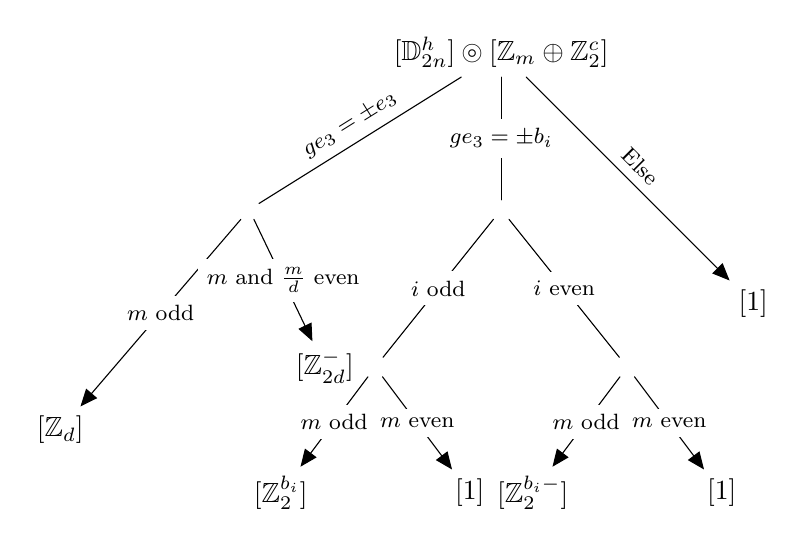
\begin{tikzpicture}[scale=0.8,line cap=round,line join=round,>=triangle 45,x=1.0cm,y=1.0cm]
  \node (root) at (0,0) {$[\DD_{2n}^h]\circledcirc [\ZZ_m\oplus \ZZ_2^c]$};

  \node (Bas1) at (-4,-2.5) {};
  \node (Bas2) at (0,-2.5) {};
  \node (Bas3) at (4,-4) {$[\1]$};
  \draw (root) -- (Bas1) node [midway,above,sloped] { \footnotesize $ge_3=\pm e_3$ };
  \draw (root) -- (Bas2) node [midway,fill=white] { \footnotesize $ge_3=\pm b_i$ };
  \draw [->] (root) -- (Bas3) node [midway,above,sloped] {{\footnotesize Else}};
  \node (Bas11) at (-7,-6) {$[\ZZ_d]$};
  \node (Bas12) at (-2.8,-5) {$[\ZZ_{2d}^-]$};
  \draw[->] (Bas1) -- (Bas11) node [midway,fill=white] {{\footnotesize $m$ odd}};
  \draw[->] (Bas1) -- (Bas12) node [midway,fill=white] {{\footnotesize $m$ and $\frac{m}{d}$ even}};
  \node (Bas21) at (-2,-5) {};
  \node (Bas22) at (2,-5) {};
  \draw (Bas2) -- (Bas21) node [midway,fill=white] {{\footnotesize $i$ odd}};
  \draw (Bas2) -- (Bas22) node [midway,fill=white] {{\footnotesize $i$ even}};
  \node (Bas211) at (-3.5,-7) {$[\ZZ_2^{b_i}]$};
  \node (Bas212) at (-0.5,-7) {$[\1]$};
  \draw[->] (Bas21) -- (Bas211) node [midway,fill=white] {{\footnotesize $m$ odd}};
  \draw[->] (Bas21) -- (Bas212) node [midway,fill=white] {{\footnotesize $m$ even}};
  \node (Bas221) at (0.5,-7) {$[\ZZ_2^{b_i-}]$};
  \node (Bas222) at (3.5,-7) {$[\1]$};
  \draw[->] (Bas22) -- (Bas221) node [midway,fill=white] {{\footnotesize $m$ odd}};
  \draw[->] (Bas22) -- (Bas222) node [midway,fill=white] {{\footnotesize $m$ even}};
\end{tikzpicture}
% Further ’tikzpicture’ environments are possible which will create further pages.
\end{document} 